\documentclass[a4paper]{article}
\usepackage{etoolbox}
\usepackage[colorlinks,bookmarksopen,bookmarksnumbered,citecolor=red,urlcolor=red]{hyperref}
\usepackage[affil-it]{authblk}
\usepackage[cm]{fullpage}
\usepackage{amsmath, amssymb, amsthm, amscd, mathtools, stmaryrd}
\usepackage{fullpage}
\usepackage{algorithm,algcompatible}
\usepackage{listings}
\usepackage{color}
\usepackage{graphicx}
\usepackage{multirow}
\usepackage{subfig}
\usepackage{mathrsfs}
\usepackage{booktabs,tabularx}
\usepackage{caption}

% For diagrams
\usepackage{tikz}
\usetikzlibrary{matrix}

%%%%%%%%% Custom math commands %%%%%%%%%
\DeclarePairedDelimiter\norm{\lVert}{\rVert}
\DeclarePairedDelimiter\jump{\llbracket}{\rrbracket}
\DeclarePairedDelimiter\avg{\{\!\!\{}{\}\!\!\}}
\DeclarePairedDelimiter{\both}{\lbrace}{\rbrace}
\renewcommand{\vec}[1]{\boldsymbol{#1}}
\newcommand{\zhat}{\hat{\vec{z}}}
\newcommand{\rhat}{\hat{\vec{r}}}
\newcommand{\ddt}[1]{\frac{\partial #1}{\partial t}}
\newcommand{\Uspace}{\mathbb{U}}
\newcommand{\Vspace}{\mathbb{V}}
\newcommand{\Wspace}{\mathbb{W}}
\newcommand{\Hdiv}{\texttt{HDiv}}
\newcommand{\Hcurl}{\texttt{HCurl}}

\newcommand{\thgsays}[1]{{\bfseries Thomas says:} {\color{blue} #1}}
\newcommand{\cjcsays}[1]{{\bfseries Colin says:} {\color{red} #1}}

\title{Code verification for the manuscript:
``Slate: extending Firedrake's domain-specific abstraction to hybridized solvers for geoscience and beyond''}

\author[$\dagger$,1]{Thomas H. Gibson}
\affil[1]{Department of Mathematics, Imperial College, South Kensington Campus, London SW7 2AZ}
\affil[$\dagger$]{Email: \texttt{t.gibson15@imperial.ac.uk}}

\date{\today}
\begin{document}

\maketitle

\section{Code verification}\label{subsec:hybridpoisson}
To verify our computed results, we now perform a simple convergence study for a model Dirichlet
problem. We seek a solution to the Poisson equation as a first-order system:
\begin{align}\label{eq:modelpoisson}
	\boldsymbol{u} + \nabla p &= 0 \text{ in } \Omega = \lbrack 0, 1\rbrack^2, \\
	\nabla\cdot\boldsymbol{u} &= f \text{ in } \Omega, \\
	p &= p_0 \text{ on } \partial\Omega_D,
\end{align}
where $f$ and $p_0$ are chosen so that the analytic solution is the sinusoid
$p(x, y) = \sin(\pi x)\sin(\pi y)$ and its negative gradient. We solve this problem
by hybridizing the mixed formulation of \eqref{eq:modelpoisson},
and employ our static condensation preconditioner described in Section
4.1.1 of the manuscript. All results were obtained in serial, with MUMPS providing the
LU factorization algorithms for the condensed trace system.

Each mesh in our convergence study is obtained by generating a quadrilateral mesh with $2^r$ cells
in each spatial direction, and dividing each quadrilateral cell into two equal simplicial elements.
Once the solutions are obtained, we compute a post-processed scalar solution using the method
described in Section 3.3.1 of the manuscript
via Slate-generated kernels. Figure \ref{fig:h-rt-conv}
displays the results for the hybridized Raviart-Thomas (RT) method. Our computations are in full agreement
with the theory.
\begin{figure}[!htbp]
	\centering
	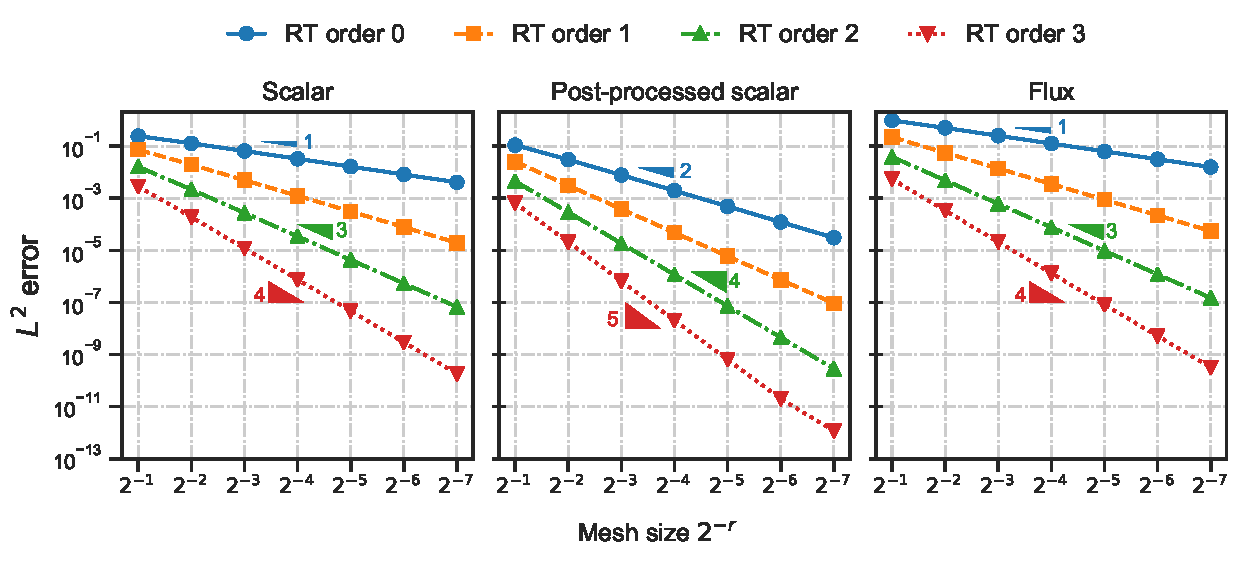
\includegraphics[width=\textwidth]{HMM/HRT-convergence}
	\caption{Error convergence rates for our implementation of the hybridized RT method of
		orders 0, 1, 2, and 3. We observe the expected rates for the scalar
		and flux solutions of the standard RT method:
		$k+1$ in the $L^2$-error for both the scalar and flux approximations.
		Additionally, we see the effects of post-processing the scalar solution, yielding
		superconvergent $k+2$ rates.}
	\label{fig:h-rt-conv}
\end{figure}

We repeat this experiment for the LDG-H method with varying choices of $\tau$
in order to verify how $\tau$ influences the convergence rates, comparing with the
expected rates for the LDG-H method given a particular order of $\tau$
(see Table \ref{table:ldg-h-rates} for a summary).
In all our experiments, we use the post-processing methods described in Sections
3.3.1 and 3.3.2 to produce approximations $p_h^\star$ and $\boldsymbol{u}_h^\star$.
Error convergence plots from our tests are shown in Figure \ref{fig:ldgh-conv} that confirm the expected
rates. This rather sensitive test verifies that our software framework is generating correct code.
\begin{table}[!htbp]
	\centering
	\caption{The expected convergence rates of the LDG-H method with a
		stability parameter $\tau$ of a particular order.}
	\begin{tabular}{ccccc}
		\hline
		parameter &
		\multicolumn{4}{c}{expected rates of convergence ($k \geq 1$)} \\
		\cline{2-5}
		$\tau$ & $\norm{p - p_h}_{L^2(\Omega)}$ &
		$\norm{\boldsymbol{u} - \boldsymbol{u}_h}_{\boldsymbol{L}^2(\Omega)}$ &
		$\norm{p - p^\star_h}_{L^2(\Omega)}$ &
		$\norm{\boldsymbol{u} - \boldsymbol{u}^\star_h}_{\boldsymbol{L}^2(\Omega)}$ \\
		\hline
		$\mathcal{O}(1)$ & $k+1$ & $k+1$ & $k+2$ & $k+1$ \\
		\hline
		$\mathcal{O}(h)$ & $k$ & $k+1$ & $k+2$ & $k+1$ \\
		\hline
		$\mathcal{O}\left(h^{-1}\right)$ & $k+1$ & $k$ & $k+1$ & $k$ \\
		\hline
	\end{tabular}
	\label{table:ldg-h-rates}
\end{table}
\begin{figure}[!htbp]
	\centering
	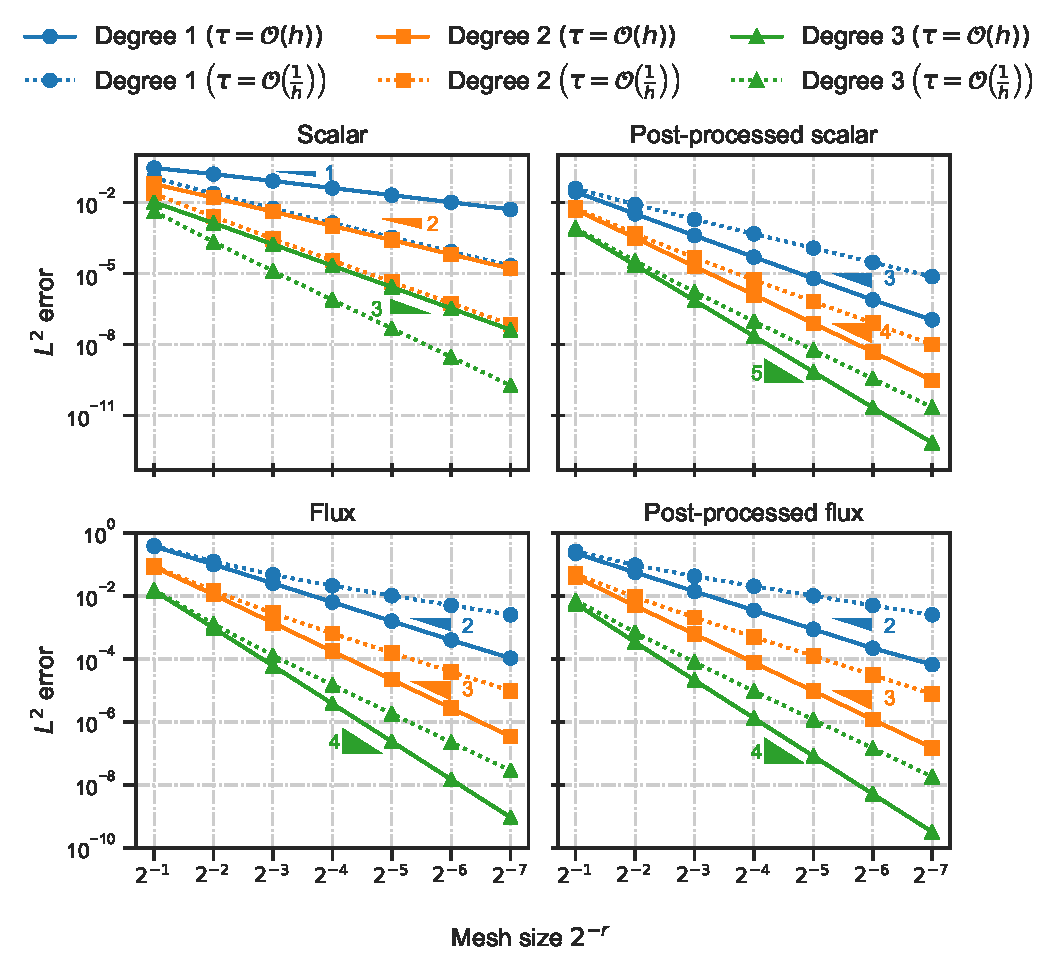
\includegraphics[width=0.8\textwidth]{LDGH/LDGH-convergence}
	\caption{Error convergence rates for our implementation of the LDG-H method with
		$\tau = h$ and $\tau = \frac{1}{h}$.
		The expected sensitivity of this discretization subject to appropriate choices of
		stabilization parameter $\tau$ is verified. We see no change in the convergence
		rates between the scalar and post-processed scalar solutions when $\tau = \frac{1}{h}$.
		Superconvergence is achieved when taking $\tau = h$. The post-processed flux rates in both
		cases match the rates of the unprocessed flux.}
	\label{fig:ldgh-conv}
\end{figure}

\end{document}